\graphicspath{{./images/}}

\chapter{Kontextabgrenzung}

\section{Fachlicher Kontext}

\begin{center}
	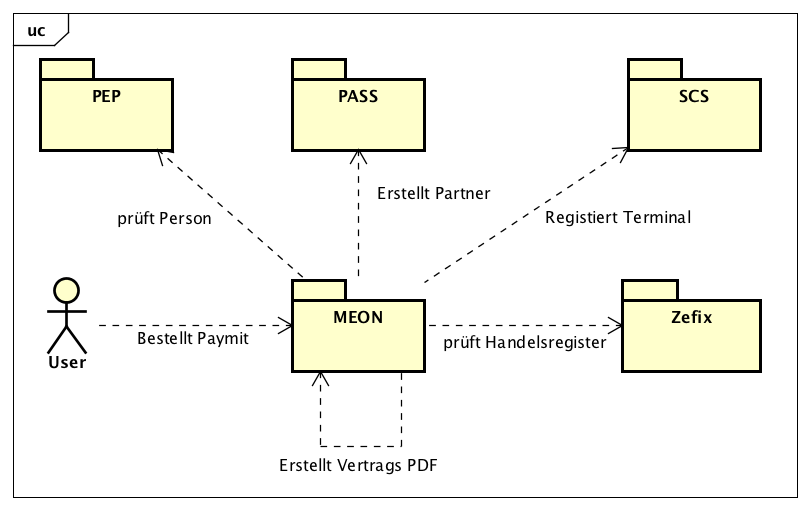
\includegraphics[scale=0.7]{kontext.png}
\end{center}


\section{Technischer Kontext}

Die Applikation MEON basiert auf dem Spring Framework als Backend und AngularJS als Frontent. Die Anwendung wird mittels der Container Technologie Docker ausgerollt. Die Details zum Deployment finden sich im Kapitel Verteilungssicht.

\section{Externe Schnittstellen}

\subsection{PASS Schnittstelle}
		
\subsubsection{Identifikation}

?

\subsubsection{Bereitgestellte Resourcen}

Zugrang zu Partnerdaten respektive die Möglichkeiten einen zu erstellen.

\subsubsection{Fehlerszenarien}

Ausfall der Datenbank
	
\subsubsection{Variabilitität und Konfigurierbarkeit}

?

\subsubsection{Qualitätseigenschaften}

Hochverfügbar da über zwei Datenzentern mittels Hot Cold gesichert
	
\subsubsection{Entwurfsentscheidungen} 

View ?

\subsubsection{Benutzungshinweise} 

	
\subsection{SCS Schnittstelle}

\subsubsection{Identifikation}

\subsubsection{Bereitgestellte Resourcen}

\subsubsection{Fehlerszenarien}

\subsubsection{Variabilitität und Konfigurierbarkeit}

\subsubsection{Qualitätseigenschaften}

\subsubsection{Entwurfsentscheidungen} 

\subsubsection{Benutzungshinweise} 


\subsection{ZEFIX Schnittstelle}

\subsubsection{Identifikation}

\subsubsection{Bereitgestellte Resourcen}

\subsubsection{Fehlerszenarien}

\subsubsection{Variabilitität und Konfigurierbarkeit}

\subsubsection{Qualitätseigenschaften}

\subsubsection{Entwurfsentscheidungen} 

\subsubsection{Benutzungshinweise} 



